\textbf{{双口RAM}}

具有两组相互独立的地址线、数据线和读/写控制线,如下图所示。由于它可以进行并行的独立操作,因此是一种高速工作的存储器。很有可能在同一时间两个端口同时操作存储器的同一存储单元,这样就发生了冲突。为了解决此问题,特设置了BUSY标志。在这种情况下,当某存储单元被某端口访问时,就对另一个端口设置BUSY延迟,另一个端口就无法访问该存储单元。

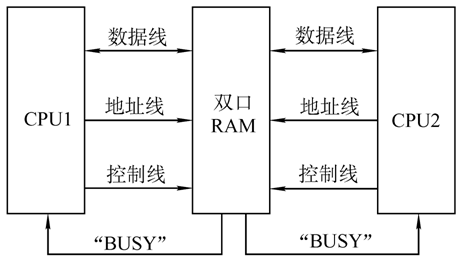
\includegraphics[width=3.69792in,height=2.12500in]{png-jpeg-pics/36B51C372D0C18E3AFC287B6D1CB8267.png}

{\textbf{单体多字存储器}}\\
单体多字存储器的\textbf{使用前提是指令和数据在主存内必须连续存放,否则效果会很差}。单体多字存储器把存储器的存储字字长增加n倍,以存放n个指令字或数据字,于是单体多字存储器的最大带宽比单体单字存储器的最大带宽提高n倍。因为程序使用指令字和数据字也存在一定的随机性,因此,一次读取的n个字很有可能是最近不需要的,正常情况下不可能达到最大带宽。{缺点:必须是凑齐了n个数据字之后才能作为一个存储字一次写入存储器。}

{\textbf{多模块存储器}}\\
多体并行存储器就是采用多个模块组成的存储器,每个模块有相同的容量和存取速度,各模块都有独立的地址寄存器、数据寄存器、地址译码器和读/写电路。多体并行存储器分为两种:高位交叉编址的多体存储器和低位交叉编址的多体存储器。\\
\textbf{1)高位交叉编址}。高位交叉编址是高位地址表示体号,低位地址来定位体内地址。按这种方式,可以在同一时间使得不同的请求源同时访问不同的体(如在某一时刻,CPU在和第0个体交换数据,而此时第1个体正在和I/O交换数据),进而实现个体的并行工作。\\
\textbf{2)低位交叉编址}。低位地址可用来表示体号,高位地址可用来定位体内地址。这样,连续地址分布在相邻的不同模块内,而同一个模块的地址都是不连续的。因此,低位交叉编址存储器可以实现多模块流水线式并行存取,大大提高存储器的带宽。\\
假设模块存取周期为T,总线传送周期为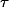
\includegraphics[width=0.09375in,height=0.07292in]{texmath/890332tau},且存储器由m个模块组成,若采用低位交叉编址的存储器,连续读取n个字所需要的时间t1=T+(n-1)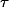
\includegraphics[width=0.09375in,height=0.07292in]{texmath/890332tau};若采用高位交叉编址的存储器,连续读取n个字所需要的时间t2=nT。\\
\textbf{注意:高位交叉编址中的并行体现在不同的请求源并行地访问不同的体;低位交叉编址中的并行体现在同一请求源并行地访问不同的体。}
